\section{Auswertung}
\label{sec:Auswertung}

$c_w = \qty{4182}{\kilo\joule\per\kilo\gram\per\kelvin}$ \cite[381]{PhyPrak}
$m_kc_k=\qty{750}{\joule\per\kelvin}
m_1= \qty{3}{\liter}
p_0= \qty{100000}{\pascal}
T_0= \qty{273.15}{\kelvin}
M= \qty{120.9}{\gram\per\mol}
\rho_0= \qty{5.51}{\kilo\gram\per\cubic\meter}
\kappa=\qty{1.14}{\watt\per\meter\per\kelvin}$
%R=8.31446261815324$

\begin{table}[H]
	\centering
	\caption{Messwerte der Wärmepumpe.}
	\label{tab:Tab1}
  \sisetup{table-format=3.2}
	\begin{tabular}{S[table-format=4.0] S S S[table-format=1.1] S[table-format=2.1] S[table-format=3.0]}
		\toprule
      {$t \mathbin{/} \si{\second}$}&{$T_1 \mathbin{/} \si{\kelvin}$}&{$T_2 \mathbin{/} \si{\kelvin}$}&{$p_a \cdot 10^{-5} \mathbin{/} \si{\pascal}$}&{$p_b \cdot 10^{-5} \mathbin{/} \si{\pascal}$} &
      {$N \mathbin{/} \si{\watt}$}\\
    \midrule
      0 & 294,15 & 293,85 & 4,8 & 4,5 & 0\\
      60 & 294,85 & 293,75 & 4,0 & 6,0 & 115\\
      120 & 296,05 & 292,65 & 4,2 & 6,5 & 120\\
      180 & 297,55 & 291,15 & 4,4 & 6,8 & 122\\
      240 & 299,05 & 289,75 & 4,4 & 7,0 & 125\\
      300 & 300,55 & 288,55 & 4,4 & 7,1 & 125\\
      360 & 302,05 & 287,45 & 4,2 & 7,5 & 122\\
      420 & 303,45 & 286,45 & 4,0 & 7,9 & 122\\
      480 & 304,85 & 285,35 & 4,0 & 8,0 & 122\\
      540 & 306,15 & 284,35 & 3,8 & 8,3 & 122\\
      600 & 307,35 & 283,45 & 3,7 & 8,8 & 122\\
      660 & 308,45 & 282,55 & 3,6 & 9,0 & 125\\
      720 & 309,65 & 281,65 & 3,5 & 9,1 & 125\\
      780 & 310,65 & 280,75 & 3,4 & 9,5 & 125\\
      840 & 311,65 & 279,85 & 3,4 & 9,7 & 125\\
      900 & 312,65 & 279,05 & 3,2 & 10,0 & 115\\
      960 & 314,45 & 278,15 & 3,2 & 10,2 & 115\\
      1020 & 314,45 & 277,35 & 3,2 & 10,2 & 115\\
      1080 & 315,25 & 276,75 & 3,0 & 10,5 & 115\\
      1140 & 316,05 & 276,05 & 3,0 & 11,0 & 115\\
      1200 & 316,75 & 275,35 & 3,0 & 11,0 & 115\\
      1260 & 317,55 & 274,75 & 2,9 & 11,2 & 115\\
      1320 & 318,95 & 274,05 & 2,8 & 11,5 & 115\\
      1380 & 318,95 & 273,45 & 2,8 & 11,5 & 115\\
      1440 & 319,55 & 272,95 & 2,7 & 11,8 & 115\\
      1500 & 320,15 & 272,45 & 2,7 & 12,0 & 115\\
      1560 & 320,75 & 271,85 & 2,7 & 12,0 & 115\\
      1620 & 321,35 & 271,35 & 2,6 & 12,1 & 110\\
      1680 & 321,95 & 270,75 & 2,6 & 12,2 & 110\\
      1740 & 322,45 & 270,35 & 2,6 & 12,3 & 110\\
      1800 & 322,95 & 269,85 & 2,5 & 12,6 & 110\\
      1860 & 323,55 & 269,85 & 2,5 & 13,0 & 110\\
    \bottomrule
  \end{tabular}
\end{table}	

\begin{figure}
  \centering
  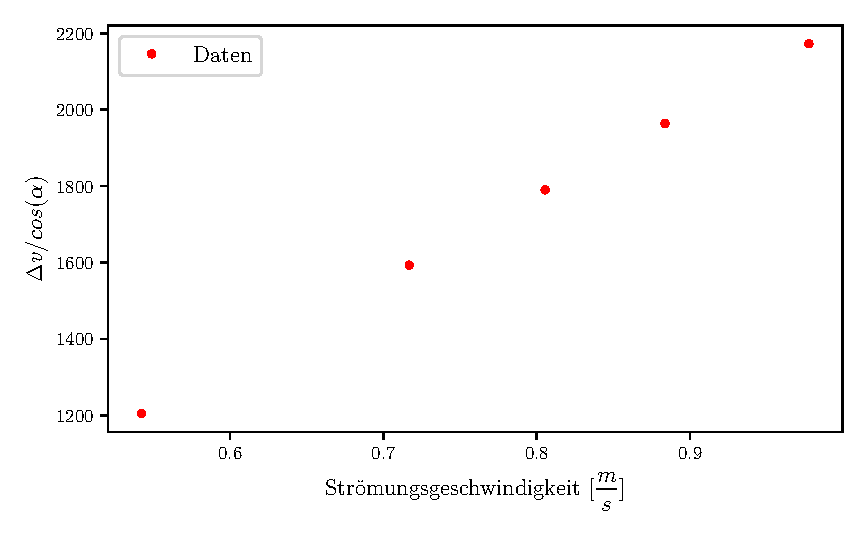
\includegraphics{plot1.pdf}
  \caption{Plot.}
  \label{fig:plot1}
\end{figure}


Die Parameter werden mithilfe von Python bestimmt und lauten für die Ausgleichskurve von $T_1$
\begin{align*}
  a&= (-5,5677 \pm 0,1998) \cdot 10^6 \si{\kelvin\per\second\squared}\\
  b&= (0,0264 \pm 0,0004) \si{\kelvin\per\second}\\
  c&= (293,37 \pm 0,15) \si{\kelvin},
\end{align*}
und für die Ausgleichskurve von $T_2$
\begin{align*}
  a&= (4,0330 \pm 0,1331) \cdot 10^6 \si{\kelvin\per\second\squared}\\
  b&= (-0,0209 \pm 0,0003) \si{\kelvin\per\second}\\
  c&= (294,56 \pm 0,10) \si{\kelvin}.
\end{align*}


\begin{table}[H]
	\centering
	\caption{Differenzenquotienten von Temperaturen $T_1$ und $T_2$ zu vier gewählten Zeitpunkten.}
	\label{tab:Tab2}
  \sisetup{table-format=1.4}
	\begin{tabular}{S[table-format=4.0] S[table-format=3.2] S@{${}\pm{}$}S S[table-format=3.2] S[table-format=3.4]@{${}\pm{}$}S}
		\toprule
      {$t \mathbin{/} \si{\second}$}&{$T_1 \mathbin{/} \si{\kelvin}$}&\multicolumn{2}{c}{$\frac{dT_1}{dt}$}&{$T_2 \mathbin{/} \si{\kelvin}$}&\multicolumn{2}{c}{$\frac{dT_2}{dt}$}\\
    \midrule
    420  & 303,45 & 0,0230 & 0,0004 & 286,45 & -0,0186 & 0,0003 \\
    840  & 311,65 & 0,0229 & 0,0004 & 279,85 & -0,0186 & 0,0003 \\
    1260 & 317,55 & 0,0228 & 0,0004 & 274,75 & -0,0187 & 0,0003 \\
    1680 & 321,95 & 0,0228 & 0,0004 & 270,75 & -0,0187 & 0,0003 \\
    \midrule
    {Mittelwert}&
    \bottomrule
  \end{tabular}
\end{table}	

\begin{table}[H]
	\centering
	\caption{Reale und ideale Güteziffer zu vier gewählten Zeitpunkten.}
	\label{tab:Tab3}
  \sisetup{table-format=1.2}
	\begin{tabular}{S[table-format=4.0] S@{${}\pm{}$}S S[table-format=2.2] S[table-format=2.1]}
		\toprule
      {$t \mathbin{/} \si{\second}$}&\multicolumn{2}{c}{Güteziffer $\nu$}&\multicolumn{2}{c}{ideale Güteziffer $\nu_{id}$}&{Abweichung $\mathbin{/} \si{\percent}$}\\
    \midrule
      420  & 2,68 & 0,10 & 17,85 & 85,0 \\
      840  & 2,67 & 0,10 &  9,80 & 72,7 \\
      1260 & 2,67 & 0,10 &  7,42 & 64,1 \\
      1680 & 2,66 & 0,10 &  6,29 & 57,7 \\
    \bottomrule
  \end{tabular}
\end{table}

Berechnung der Güteziffer mit Formeln blabla
wobei N gemittelt aus Tab1 zu $N_m= (114 \pm 4) \si{\watt}$


\begin{figure}
  \centering
  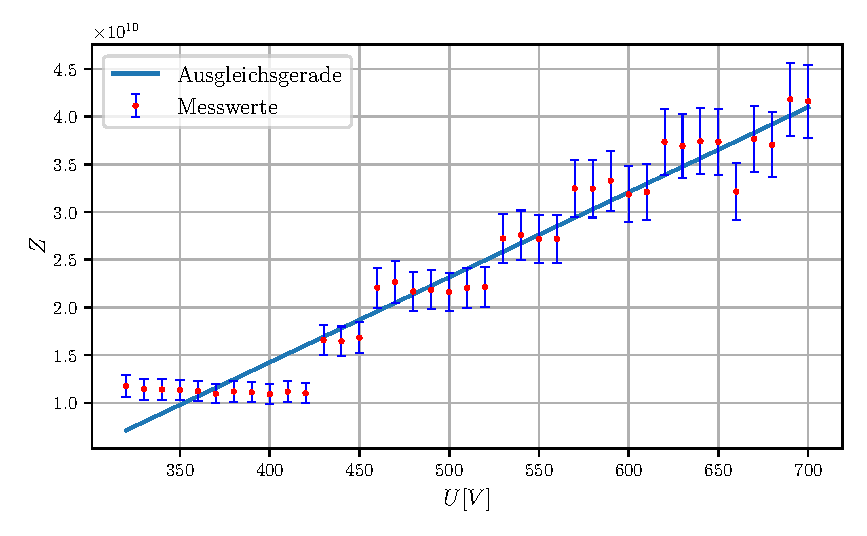
\includegraphics{plot2.pdf}
  \caption{Plot.}
  \label{fig:plot2}
\end{figure}
\begin{align}
  a&= (-2621.10 \pm 97.45) \si{\kelvin}
  b&= (10.67 \pm 0.31)
  L&= (21793.07 \pm 810.28) \si{\joule\per\mol}.
\end{align}

\begin{table}[H]
	\centering
	\caption{Massendurchsatz zu vier gewählten Zeitpunkten.}
	\label{tab:Tab4}
  \sisetup{table-format=1.4}
	\begin{tabular}{S[table-format=4.0] S[table-format=3.4]@{${}\pm{}$}S[table-format=1.4] S[table-format=3.2]@{${}\pm{}$} S[table-format=1.2]}
		\toprule
      {$t \mathbin{/} \si{\second}$}&\multicolumn{2}{c}{$\frac{dm}{dt} \mathbin{/} \si{\mol\per\second}$}&\multicolumn{2}{c}{$\frac{dm}{dt} \mathbin{/} \si{\gram\per\second}$}\\
    \midrule
      420  -0,0113 & 0,0005 & -1,37 & 0,05\\
      840  -0,0114 & 0,0005 & -1,37 & 0,05\\
      1260 -0,0114 & 0,0005 & -1,38 & 0,05\\
      1680 -0,0114 & 0,0005 & -1,38 & 0,05\\
    \bottomrule
  \end{tabular}
\end{table}

\begin{table}[H]
	\centering
	\caption{Dichte und mechanische Leistung des Kompressors zu vier gewählten Zeitpunkten.}
	\label{tab:Tab5}
  \sisetup{table-format=1.4}
	\begin{tabular}{S[table-format=4.0] S[table-format=3.4]@{${}\pm{}$}S[table-format=1.4] S[table-format=3.2]@{${}\pm{}$} S[table-format=1.2]}
		\toprule
      {$t \mathbin{/} \si{\second}$}&{$\rho \mathbin{/} \si{\kilo\gram\per\cubic\meter}$}&\multicolumn{2}{c}{$N_{mech} \mathbin{/} \si{\watt}$}\\
    \midrule
      420  & 21,02 & 16,2 & 0,6\\
      840  & 18,29 & 25,1 & 1,0\\
      1260 & 15,89 & 32,4 & 1,3\\
      1680 & 14,45 & 37,0 & 1,5\\
      \bottomrule
    \end{tabular}
  \end{table}

